\section{Περιγραφή δεδομένων}
\subsection{Ανάλυση καταναλώσεων}
\subsection{Μοντελοποίηση εποχιακών δεικτών}
Για βαθύτερη κατανόηση των χρονοσειρών γίνεται εκτίμηση της εποχιακής και μη εποχιακής καταναλωτικής τάσης με τη χρήση παραμετρικών μοντέλων. Με αυτό τον τρόπο θα καταστεί δυνατή η παρατήρηση της επαναληψιμότητας και των μορφών των καταναλώσεων. Για να γίνει αυτό χρησιμοποιείται αρχικά ο αλγόριθμος K-Means για την ομαδοποίηση των καταναλωτών σε τέσσερις συστάδες βάση του ετήσιου μέσου όρου καθενός. Στη συνέχεια δημιουργείται ένα προφίλ κατανάλωσης για κάθε συστάδα βρίσκοντας το μέσο ημερήσιο όρο κατανάλωσης. Χρειάστηκαν 2000 καταναλωτές για αυτή την ανάλυση με περισσότερους  1800 να ομαδοποιούνται σε δύο ομάδες υποδεικνύοντας προφίλ οικιακών καταναλωτών.
\subsubsection{Ανάλυση Παλινδρόμησης}
Σκοπός, λοιπόν αυτού του μέρους είναι να γίνει στατιστική μελέτη του πολυωνυμικού μοντέλου στα δεδομένα μας και να δούμε αν οι χρονοσειρές κάθε συστάδας μπορούν να περιγραφούν  με πολυώνυμο δευτέρου βαθμού. \cite{mathworkstrend}
\begin{center}
$T_t=\beta_0 + \beta_1t + \beta_2t^2$
\end{center}

\begin{figure}[ht!]
\centering
\includegraphics[width=180mm, height=120mm]{../../plots/Trend_estimation/quadratic_Trend_ALL.png}
\caption{Εφαρμογή πολυωνύμου δευτέρου  βαθμού}
\label{fig:quadratic trend}
\end{figure}


Όπως φαίνεται στο Σχήμα \ref{fig:quadratic trend} οι συστάδες μπορούν να χαρακτηριστούν από μια παραβολική καμπύλη με θετικό συντελεστή μεγιστοβάθμιου όρου.
\begin{itemize}
\item Η συστάδα 1 αποτελείται από 792 καταναλωτές και έχει η παραβολική καμπύλη τάσης λαμβάνει ελάχιστη τιμή την 189η μέρα του έτους.
\item Η συστάδα 2 αποτελείται από 81 καταναλωτές και έχει η παραβολική καμπύλη τάσης λαμβάνει ελάχιστη τιμή την 206η μέρα του έτους. 
\item Η συστάδα 3 αποτελείται από 81 καταναλωτές και έχει η παραβολική καμπύλη τάσης λαμβάνει ελάχιστη τιμή την 201η μέρα του έτους.
\item Η συστάδα 4 αποτελείται από 81 καταναλωτές και έχει η παραβολική καμπύλη τάσης λαμβάνει ελάχιστη τιμή την 194η μέρα του έτους.
\end{itemize}

Εύκολα, λοιπόν, βγάνει το συμπέρασμα πως οι οικιακοί καταναλωτές έχουν την τάση να έχουν πιο ομοιόμορφα κατανεμημένα την παραβολική καμπύλη, ενώ οι επιχειρήσεις έχουν μεγαλύτερο βαθμό τυχαιότητας και λιγότερο συμμετρική καμπύλη ως προς το ελάχιστο σημείο της.
\subsubsection{Εκτίμηση εποχιακών δεικτών}
Αρχικά για την εκτίμηση των εποχιακών δεικτών απαιτείται η αφαίρεση του πολυώνυμου δευτέρου βαθμού από τις χρονοσειρές των ομάδων.\cite{timeseriesanalysis} Δεδομένης της μικρής διάρκειας των καταναλώσεων (1 έτος) καθίσταται αδύνατη η εξαγωγή εποχιακών δεικτών ανά μήνα έτους ή ανά εποχή έτους. Για αυτό το λόγο οι εποχιακοί δείκτες μεταφέρθηκαν ανά ημέρα της εβδομάδας ή ανά ημέρα του μήνα. Για την πρώτη περίπτωση οι δείκτες αναφέρονται στις ημέρες κάθε εβδομάδας, ενώ για την δεύτερη αναφέρονται στις ημέρες κάθε μήνα δημιουργώντας 7 ή 30 δείκτες αντίστοιχα. Για την εβδομαδιαία εποχιακότητα έχω τις παρακάτω καμπύλες για κάθε ομάδα.
\subsubsection{Εκτίμηση με διαστήματα ημέρας ανά εβδομάδα}
Από την εβδομαδιαία εποχιακότητα λοιπόν εύκολα κάποιος αντιλαμβάνεται πως ανάλογα με τον τύπο των καταναλωτών οι μέρες που έχουμε μέγιστη και ελάχιστη κατανάλωση διαφέρουν ριζικά. Η πρώτη μέρα του έτους για το έτος που μελετάμε είναι Πέμπτη. Ειδικότερα:
\begin{itemize}
\item Για τους καταναλωτές συστάδας 1 (οικιακοί καταναλωτές) έχουμε ελάχιστες καταναλώσεις τις Πέμπτες.
\item Για τους καταναλωτές συστάδας 2 (επιχειρήσεις) έχουμε ελάχιστες καταναλώσεις τα Σάββατα.
\item Για τους καταναλωτές συστάδας 3 (οικιακοί καταναλωτές) έχουμε ελάχιστες καταναλώσεις τις Τρίτες.
\item Για τους καταναλωτές συστάδας 4 (επιχειρήσεις) έχουμε ελάχιστες καταναλώσεις τα Σάββατα.
\end{itemize}
\newpage
\begin{figure}[ht!]
\centering
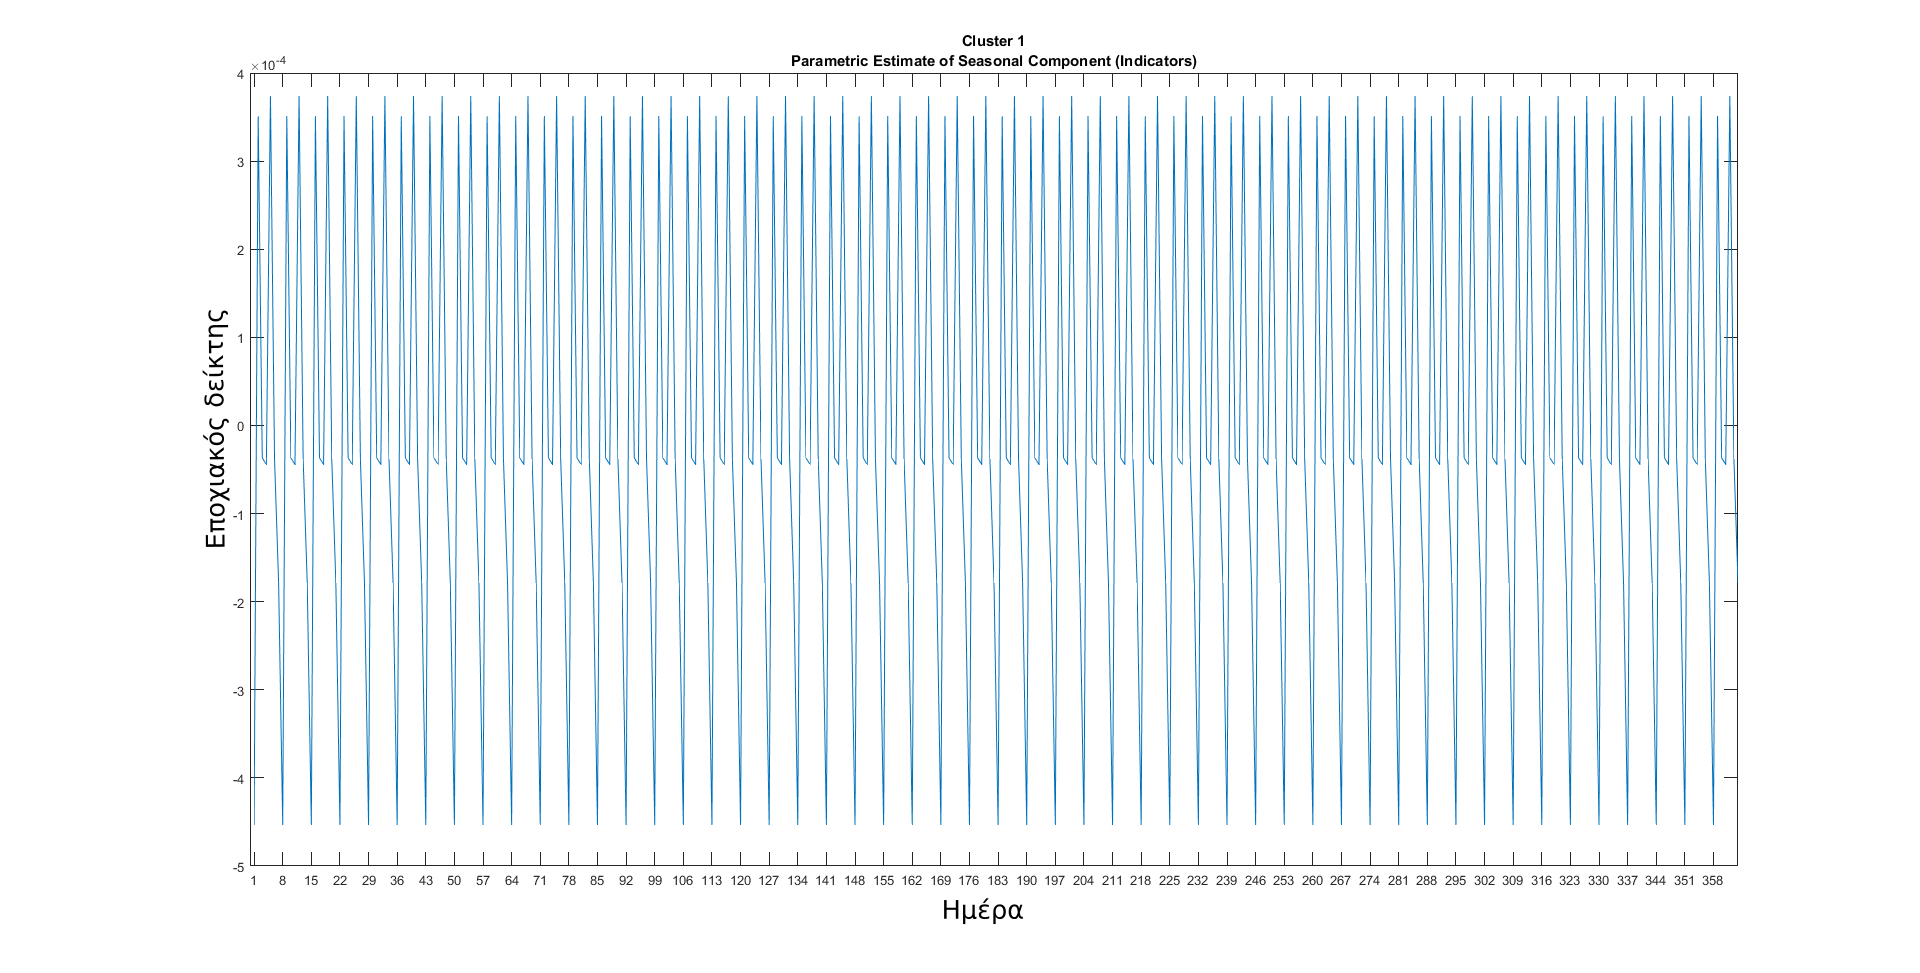
\includegraphics[width=180mm, height=100mm]{../../plots/Trend_estimation/seasonal_1.png}
\caption{Εβδομαδιαία εποχιακότητα ομάδας 1}
\label{fig:season 1}
\end{figure}
\begin{figure}[ht!]
\centering
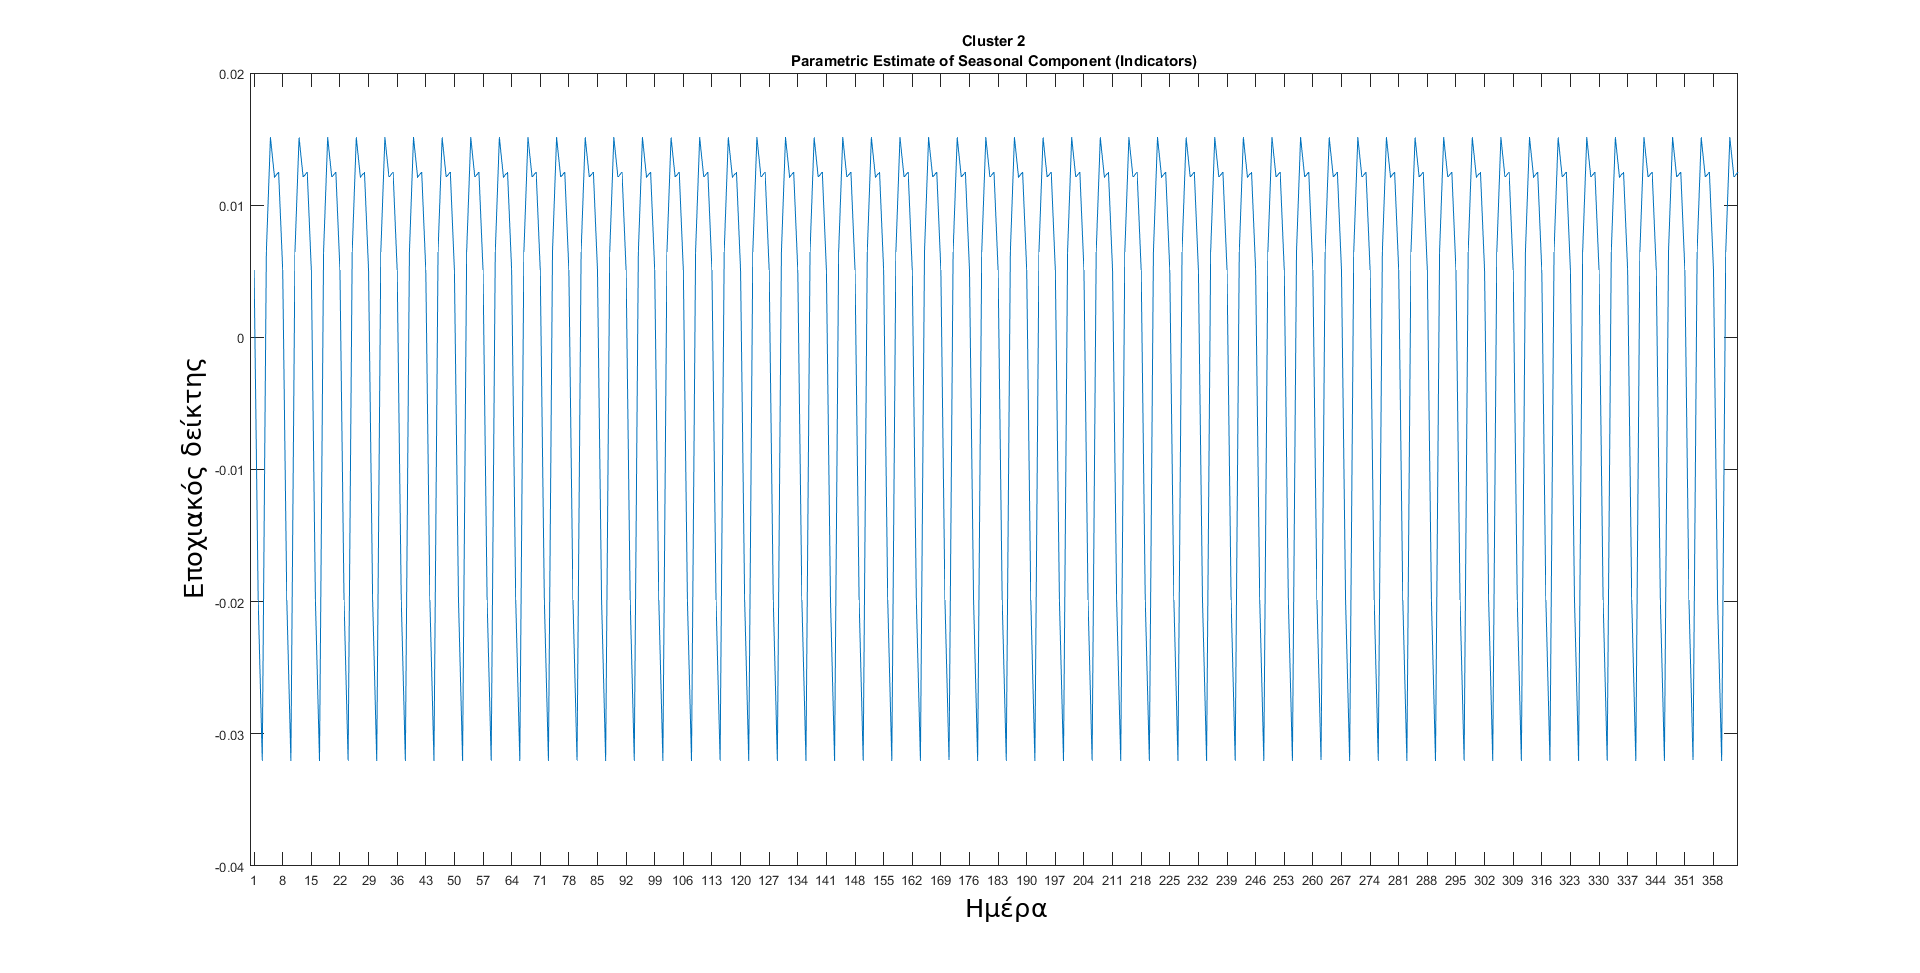
\includegraphics[width=180mm, height=100mm]{../../plots/Trend_estimation/seasonal_2.png}
\caption{Εβδομαδιαία εποχιακότητα ομάδας 2}
\label{fig:season 2}
\end{figure}
\begin{figure}[ht!]
\centering
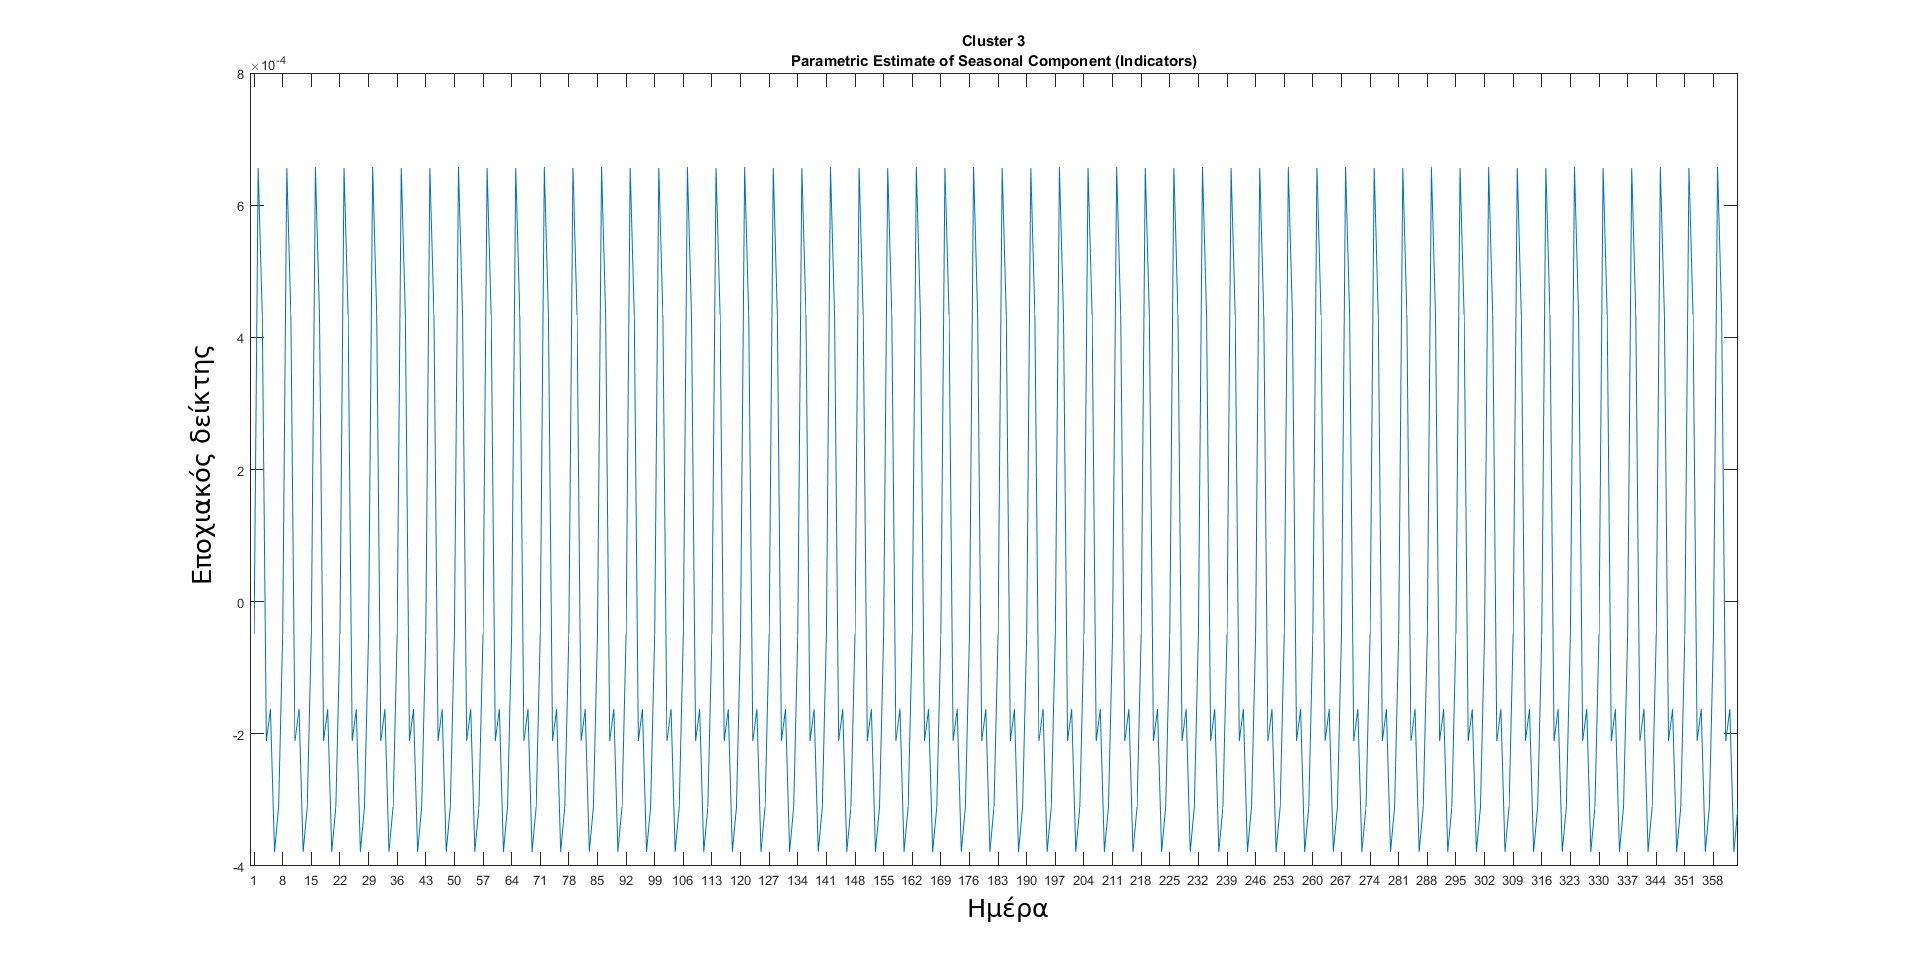
\includegraphics[width=180mm, height=100mm]{../../plots/Trend_estimation/seasonal_3.png}
\caption{Εβδομαδιαία εποχιακότητα ομάδας 3}
\label{fig:season 3}
\end{figure}
\begin{figure}[ht!]
\centering
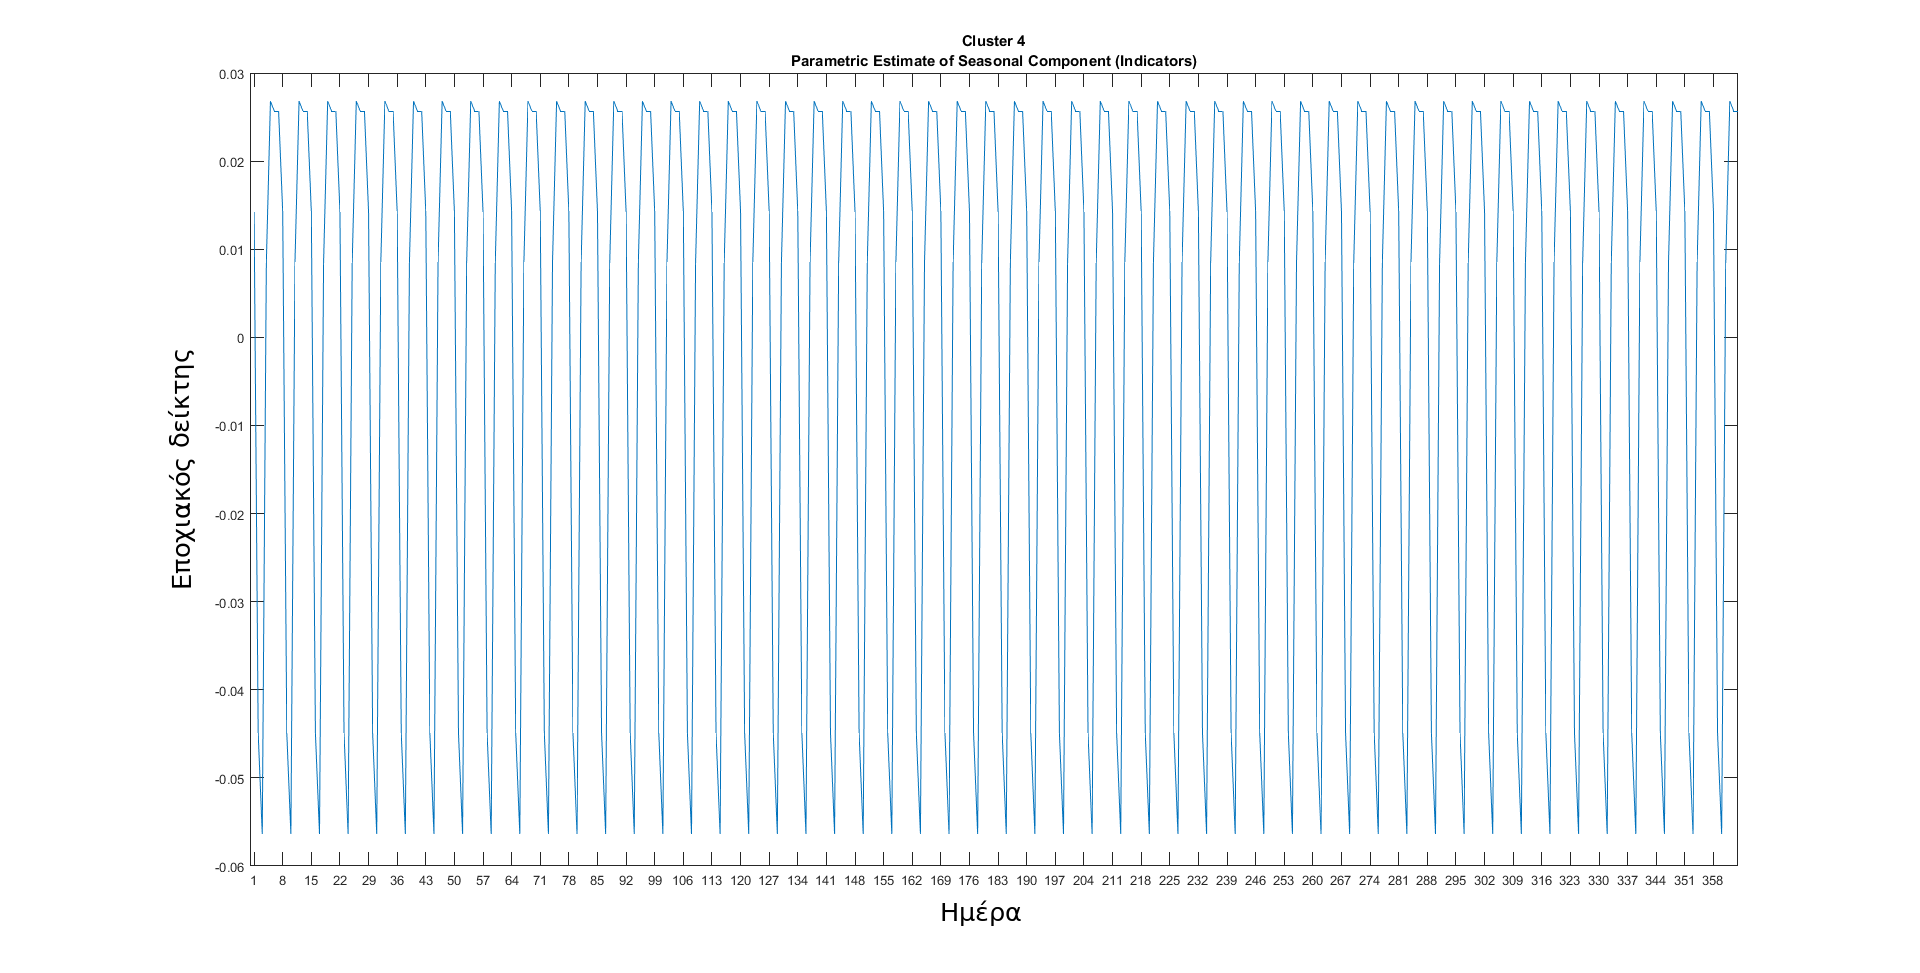
\includegraphics[width=180mm, height=100mm]{../../plots/Trend_estimation/seasonal_4.png}
\caption{Εβδομαδιαία εποχιακότητα ομάδας 4}
\label{fig:season 4}
\end{figure}
\subsubsection{Εκτίμηση σε διαστήματα ημέρας ανά μήνα}
Το διάστημα ενός μήνα αφήνει μεγαλύτερα περιθώριο εποπτείας της χρονοσειράς, ενώ ταυτόχρονα δημιουργεί αποτελέσματα με μεγαλύτερη συνοχή. Από την άλλη πλευρά οι 12 μήνες του έτους δεν μπορούν να εξάγουν πολύ ασφαλή δεδομένα αν συγκριθούν με τις 52 εβδομάδες.


Από την μηνιαία εποχιακότητα γίνεται εύκολα αντιληπτό πως ανάλογα με τον τύπο των καταναλωτών οι μέρες που έχουμε μέγιστη και ελάχιστη κατανάλωση διαφέρουν ριζικά. Ειδικότερα:
\begin{itemize}
\item Για τους καταναλωτές συστάδας 1 (επιχειρήσεις) έχουμε ελάχιστες καταναλώσεις στις 30 του μηνός.
\item Για τους καταναλωτές συστάδας 2 (οικιακοί καταναλωτές) έχουμε ελάχιστες καταναλώσεις στις 15 του μηνός.
\item Για τους καταναλωτές συστάδας 3 (οικιακοί καταναλωτές) έχουμε ελάχιστες καταναλώσεις στις 15 του μηνός.
\item Για τους καταναλωτές συστάδας 4 (επιχειρήσεις) έχουμε ελάχιστες καταναλώσεις στις 3 του μηνός.
\end{itemize}
\begin{figure}[ht!]
\centering
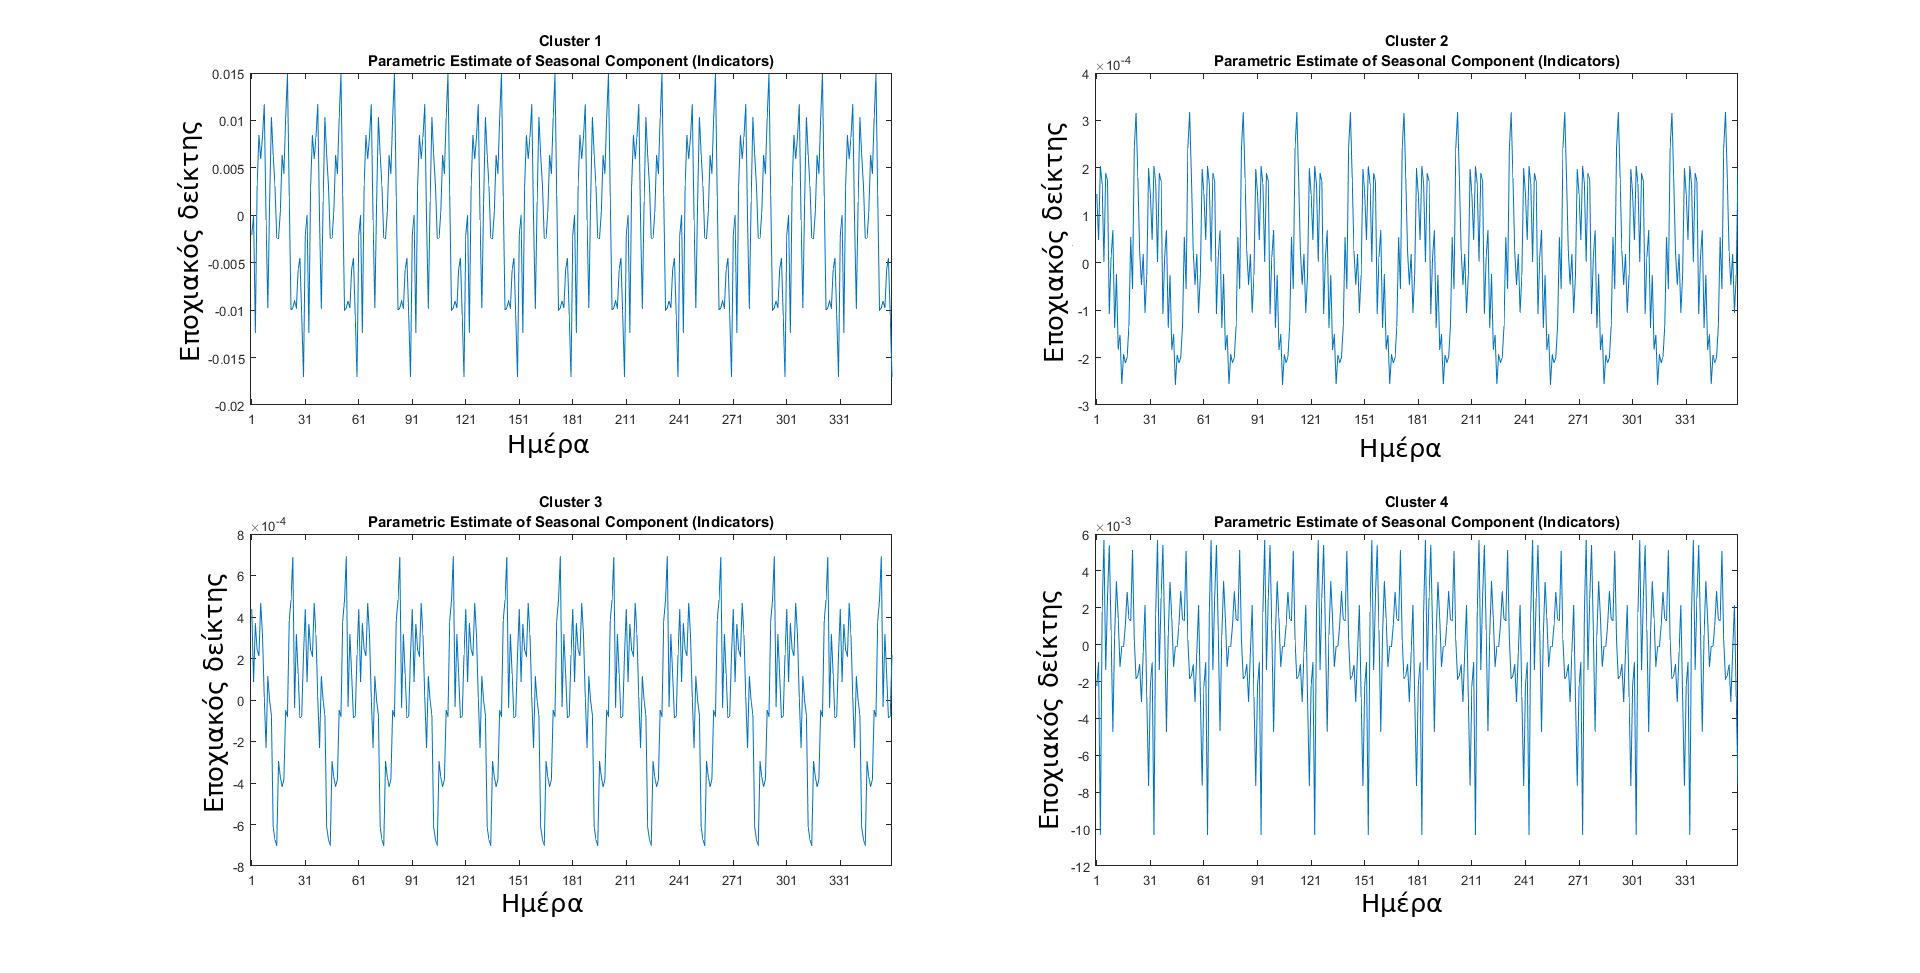
\includegraphics[width=180mm, height=120mm]{../../plots/Trend_estimation/seasonal_month_ALL.png}
\caption{Μηνιαία εποχιακότητα}
\label{fig:season daypermonth}
\end{figure}

\subsubsection{Αφαίρεση εποχιακών δεικτών}
Σε αυτό το σημείο είναι σημαντικό να παρατηρηθεί η κατανάλωση χωρίς τους εποχιακούς δείκτες. Με αυτό τον τρόπο καθίσταται ευκολότερη η θεώρηση της μορφής των κυματομορφών και η σύγκρισή τους με τις αρχικές καταναλώσεις του πρώτου μέρους. Αφαιρώντας τα εποχιακά χαρακτηριστικά οι καμπύλες πλησιάζουν περισσότερο στην παραβολική συνάρτηση. Έτσι η καταναλωτική τους τάση χωρίς τους εποχιακούς δείκτες γίνεται πιο έντονη και ευδιάκριτη.
\begin{figure}[ht!]
\centering
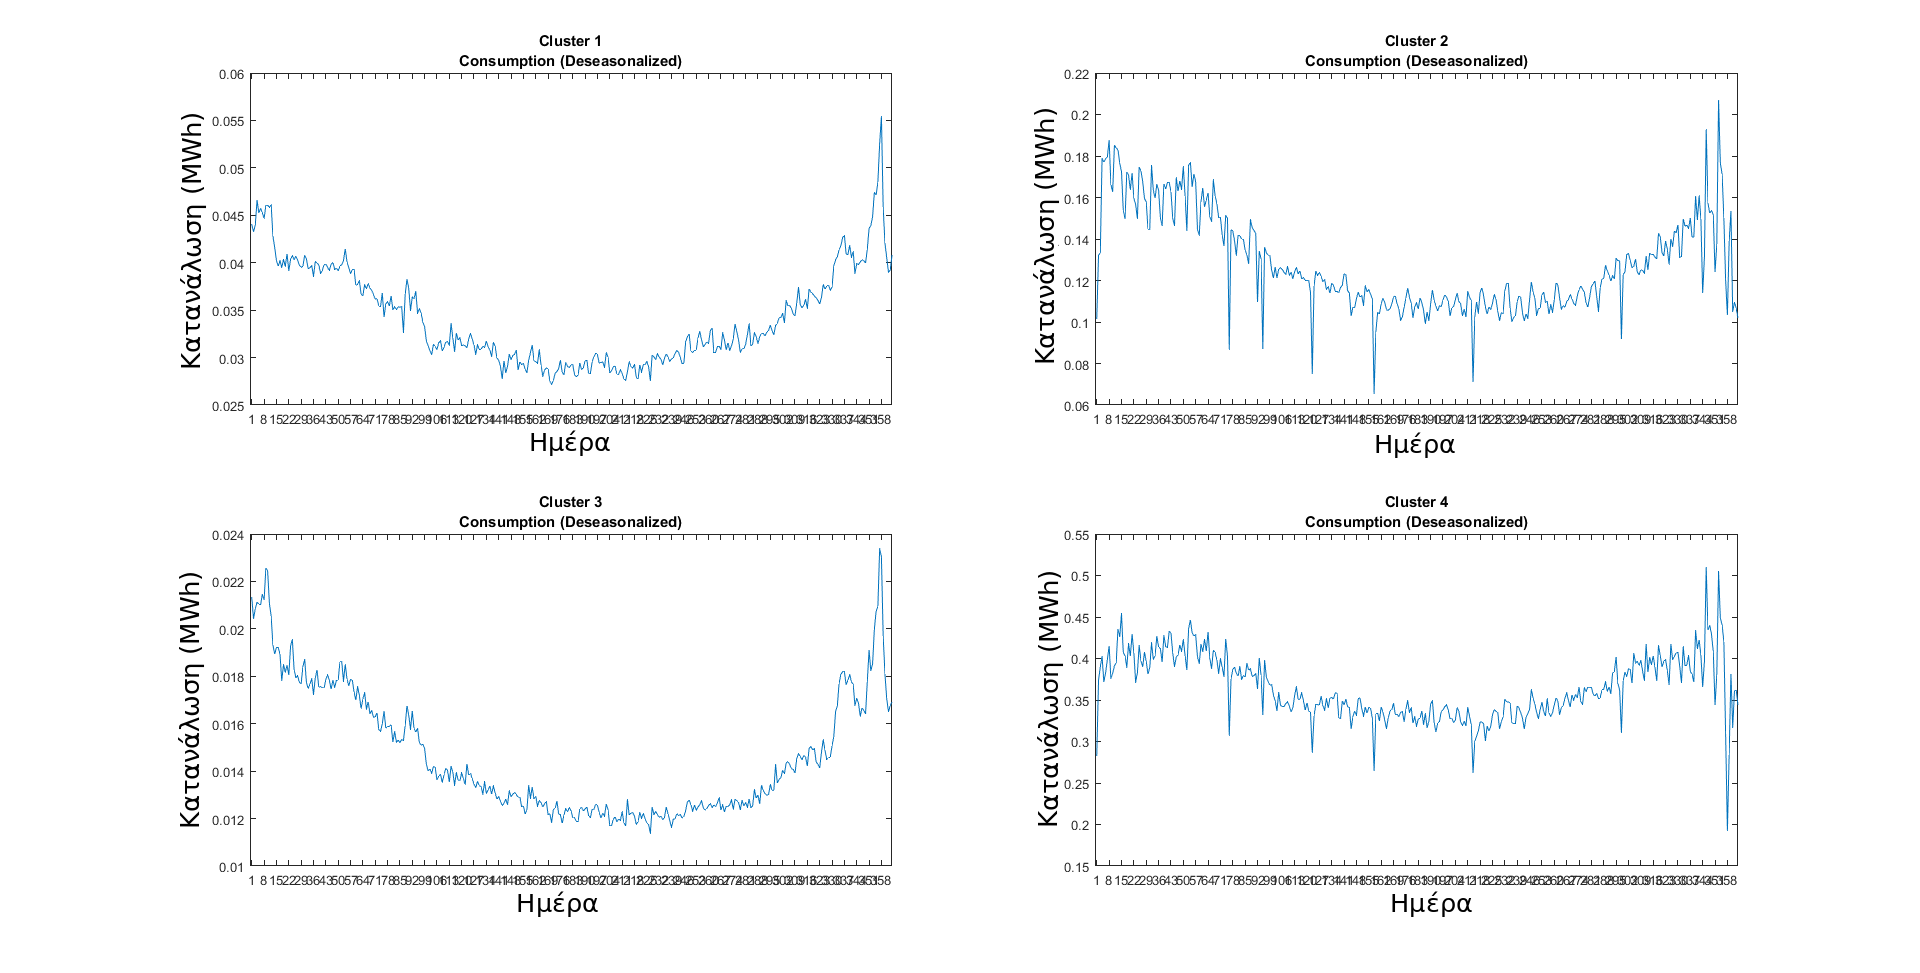
\includegraphics[width=180mm, height=120mm]{../../plots/Trend_estimation/Deseasonalized_ALL.png}
\caption{Κατανάλωση χωρίς εποχιακούς δείκτες ανά εβδομάδα}
\label{fig:deseason week}
\end{figure}
\newpage

\begin{figure}[ht!]
\centering
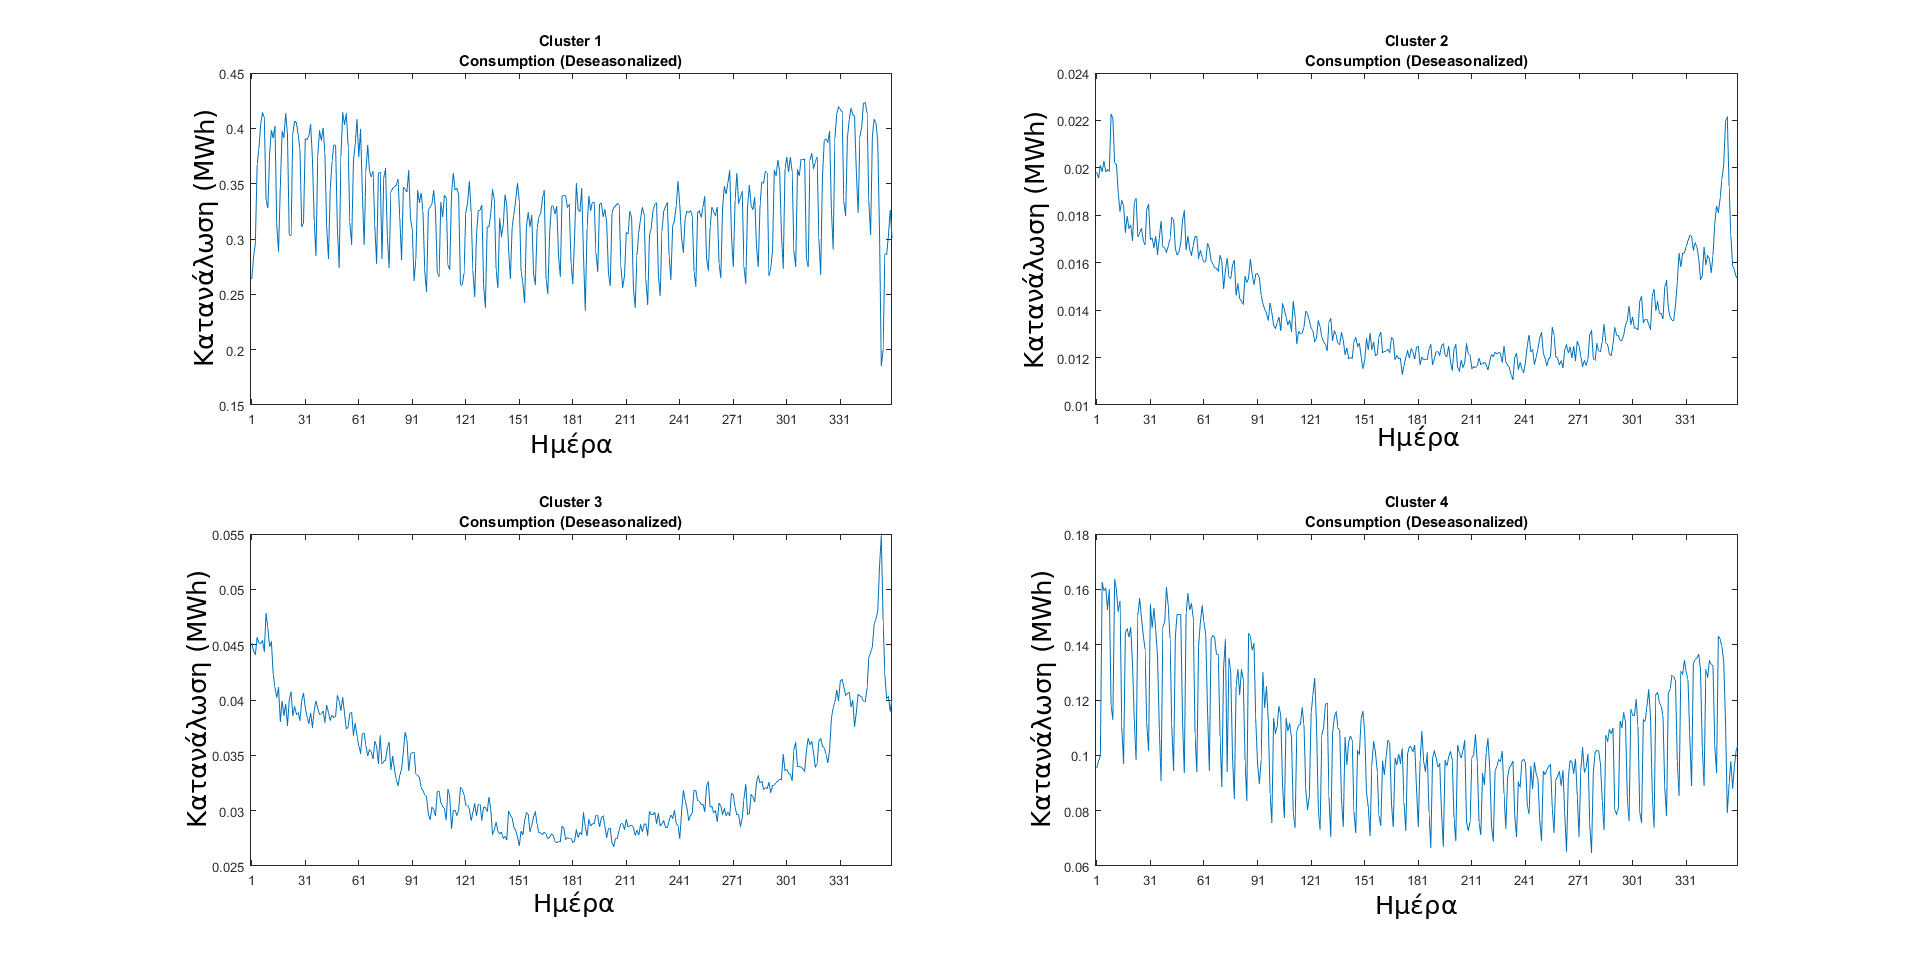
\includegraphics[width=180mm, height=120mm]{../../plots/Trend_estimation/Deseasonalized_month_ALL.png}
\caption{Κατανάλωση χωρίς εποχιακούς δείκτες ανά μήνα}
\label{fig:deseason month}
\end{figure}

\subsubsection{Εκτίμηση ακανόνιστης συνιστώσας}
Τέλος έχει ενδιαφέρουν να δούμε το βαθμό της τυχαιότητας που έχουμε στις καταναλώσεις των συστάδων που δημιουργήθηκαν. Αυτό επιτυγχάνεται αφαιρώντας την εποχιακή χρονοσειρά και την καταναλωτική τάση της αρχικής χρονοσειράς. Με αυτό τον τρόπο γίνεται σαφές ότι παρόλο την εποχιακότητα και την τάση οι χρονοσειρές έχουν αισθητό τυχαίο παράγοντα. Η αφαίρεση δημιουργεί αλλαγές στο επίπεδο της χεονοσειράς, σταθεροποιώντας έτσι το μέσο όρο της. Γίνεται αντιληπτό πως έχουν μη προβλέψιμα πρότυπα  τουλάχιστον με δεδομένα διάρκειας ενός έτους. Τέτοιου τύπου δεδομένα λέγενται στατικές χρονοσειρές.\cite{stationarity}
\begin{figure}[ht!]
\centering
\includegraphics[width=180mm, height=100mm]{../../plots/Trend_estimation/irregular_component_all.png}
\caption{Εκτίμηση ακανόνιστης συνιστώσας με εβδομαδιαία εποχιακότητα}
\label{fig:irregular week}
\end{figure}

\newpage
\begin{figure}[ht!]
\centering
\includegraphics[width=180mm, height=100mm]{../../plots/Trend_estimation/irregular_component_month_all.png}
\caption{Εκτίμηση ακανόνιστης συνιστώσας με μηνιαία εποχιακότητα}
\label{fig:irregular month}
\end{figure}
\subsubsection{Εξερεύνηση ημερών με χαμηλές καταναλώσεις}
Για να αντληθούν περαιτέρω χαρακτηριστικά των χρονοσειρών χρειάστηκε η υλοποίηση αλγορίθμου με διπλή συσταδοποίηση. Σύμφωνα με τον αλγόριθμο πρώτα συσταδοποιούνται οι καταναλωτές με βάση την ημερήσια κατανάλωση, εν συνεχεία για κάθε συστάδα δημιουργείται νέα ομαδοποίηση με βάση την ομοιότητα κάθε ημερήσιας κατανάλωσης. Με αυτό τον τρόπο μπορεί να παρατηρηθεί ποιες μέρες όμοιων καταναλωτών έχουν παρόμοιες καταναλώσεις. Καθίσταται έτσι εφικτό, να φιλτράρουμε από τα δεδομένα μας μέρες με χαμηλή κατανάλωση που γνωρίζουμε πως θα δυσκόλευαν το πρόβλημα της ταξινόμησης σε αληθή και αλλοιωμένα δεδομένα.

Τα αποτελέσματα του αλγορίθμου έδειξαν πως μόνο τα Σάββατα μιας συστάδας εμφανίζουν έντονη ομοιότητα οικιακών καταναλώσεων. Οι Κυριακές κατά κύριο λόγο συσταδοποιούνται με την υπόλοιπη εβδομάδα δημιουργώντας την εβδομαδιαία τάση, γεγονός που δείχνει πως για τους περισσότερους καταναλωτές η Κυριακή είναι εργάσιμη ημέρα. Παράλληλα, παρατηρείται πως ανά περιόδους οι καταναλώσεις δημιουργούν νέες συστάδες αφήνοντας μόνο τα Σάββατα να σπάνε την συνεχόμενη συσταδοποίηση. Στον Πίνακα \ref{tab:double clustering} φαίνεται πως ακόμη και στα Σάββατα δεν έχουμε απολύτως γεμάτες συστάδες.

\begin{table}[ht!]
\centering
\begin{tabular}{ |c||c|c|c|c|  }
 \hline
 \multicolumn{5}{|c|}{Συστάδες Καταναλωτών} \\
 \hline
 Συστάδες Σαββάτου  & Συστάδα 1& Συστάδα 2 &Συστάδα 3 &Συστάδα 4\\
 \hline
 Συστάδα 1 & 0  & 24 & 30 & 19\\
 Συστάδα 2 & 9  & 11 & 0  & 15\\
 Συστάδα 3 & 0  & 9  & 0  & 0\\
 Συστάδα 4 & 42 & 0  & 0  & 0\\
 Συστάδα 5 & 0  & 2  & 0  & 0\\
 Συστάδα 6 & 0  & 4  & 0  & 7\\
 Συστάδα 7 & 0  & 1  & 21 & 10\\
 \hline
\end{tabular}
\caption{Έλεγχος συσταδοποίησης Σαββάτου}
\label{tab:double clustering}
\end{table}

\subsubsection{Παρατηρήσεις}
Τα εμφανή χαρακτηριστικά εποχιακότητας και η εφαρμογή πολυωνύμου δευτέρου βαθμού στις χρονοσειρές θέτει καλό υποψήφιο τα μοντέλα πρόβλεψης χρονοσειρών. Με ένα τέτοιο σύστημα θα δημιουργείται μια πρόβλεψη κατανάλωσης από έμπιστους καταναλωτές για κάποιο χρονικό διάστημα. Εν συνεχεία θα αλλοιώνονται τα χαρακτηριστικά κάποιου μέρους των καταναλωτών και θα ελέγχεται αν ο αλγόριθμος μπορεί να διαχωρίσει τις αλλοιωμένες τιμές από αυτές που προέβλεψε.

\section{Προεπεξεργασία και καθάρισμα δεδομένων}
\section{Προσομοίωση απάτης}
\subsection{Τύποι απάτης}
